\subsection*{Multiple Access}
\textbf{Time Division Duplex TDD:}

The duplexer is a switch allowing to
separate transmit (Tx) and receive (Rx).It is placed between the antenna and
amplifiers. It is simple but only allows a half-duplex communication.

\textbf{Frequency Division Duplex FDD:}

A diplexer is a dual filter that split Tx and Rx in two
frequency channels. We can compare it to frequency multiplexer. It allows full duplex transmission.

\textbf{Carrier Sense Multiple Access CSMA:}

The idea is to listen to the channel before transmitting.
The disadvantage of this system is the potential collision occurring when two transmitters
start to emit at the same time.

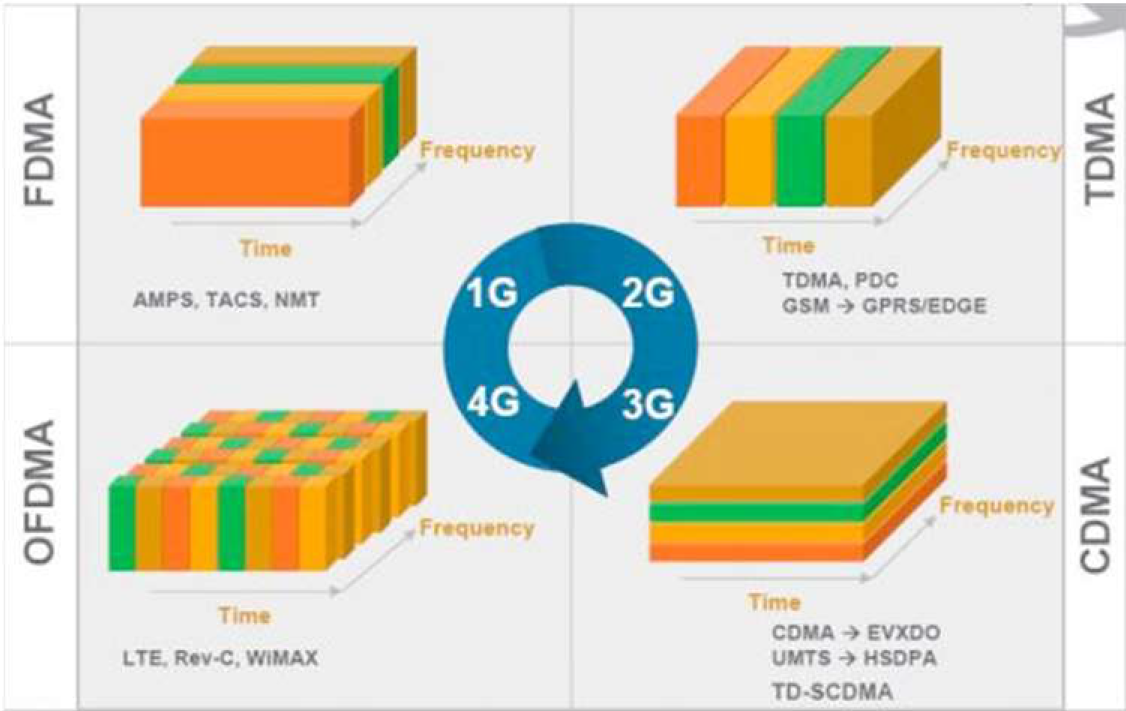
\includegraphics[width=\columnwidth]{images/multiple_access_comparison.png}

% \setlength{\intextsep}{-5pt}
% \begin{wrapfigure}{r}{0.3\textwidth}
%     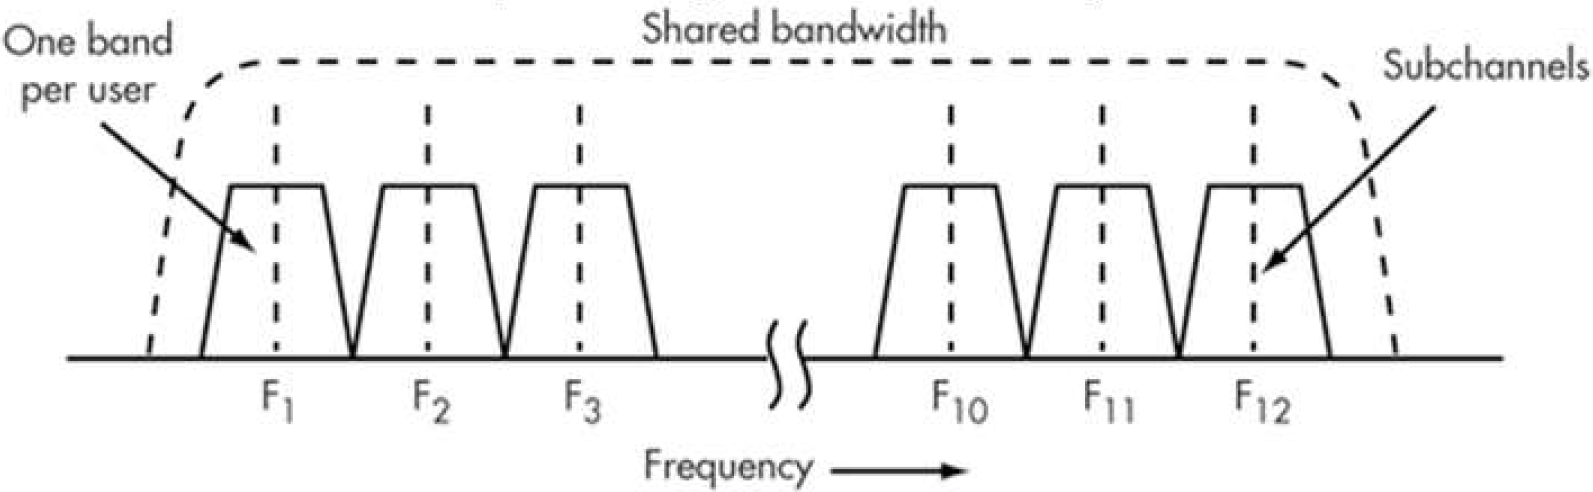
\includegraphics[width=\linewidth]{images/fdma.png}
% \end{wrapfigure}
\textbf{Frequency Division Multiple Access FDMA:}

Used in 1G. Allocation of
one frequency channel per user. Drawbacks: Number of users limited by the available bandwidth.
If one user is alone, he cannot use all the bandwidth available.

% \needspace{5\baselineskip}
% \begin{wrapfigure}{r}{0.2\textwidth}
%     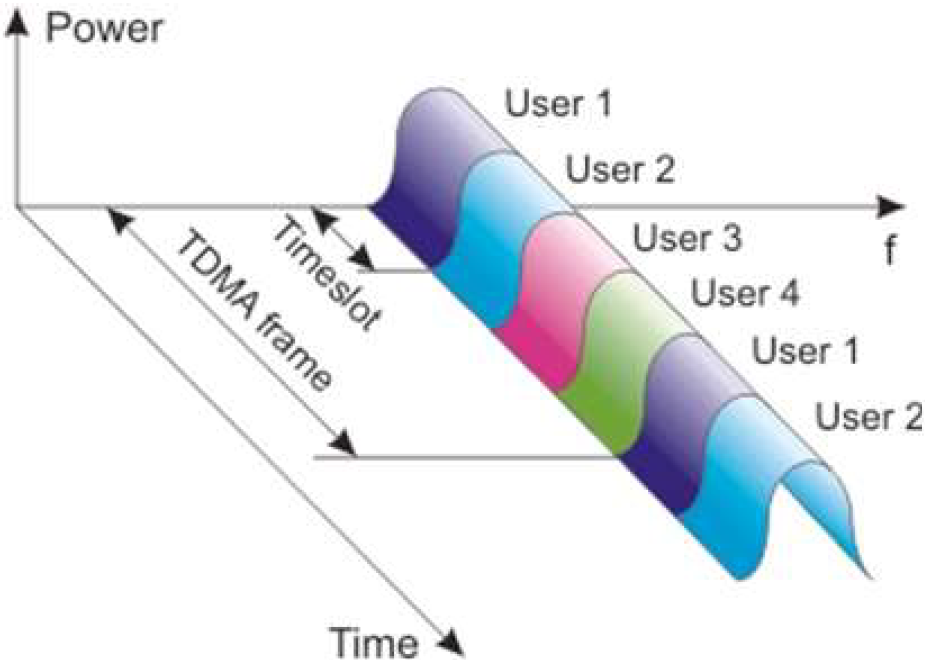
\includegraphics[width=\linewidth]{images/tdma.png}
% \end{wrapfigure}
\textbf{Time Division Multiple Access TDMA:}

Used in 2G. Allocation of one time slot per user.
Drawbacks: Time sensitive. Accurate synchronization is required to avoid overlap.\\

% \needspace{5\baselineskip}
% \begin{wrapfigure}{r}{0.3\textwidth}
%     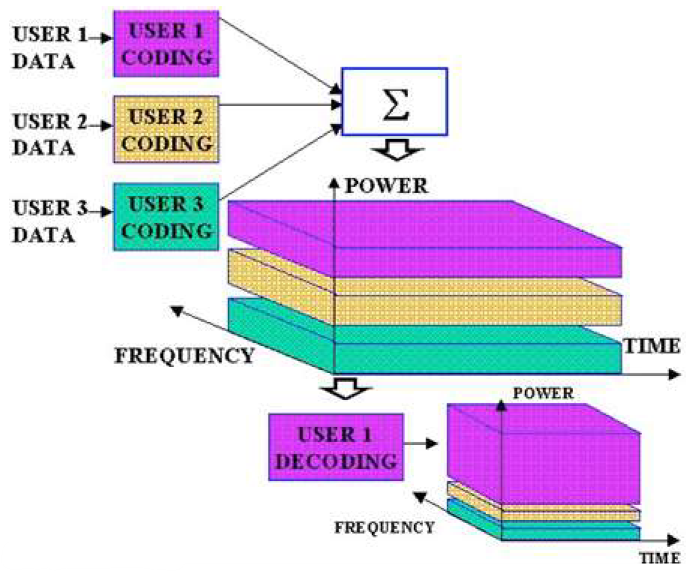
\includegraphics[width=\linewidth]{images/cdma.png}
% \end{wrapfigure}
\textbf{Code Division Multiple Access CDMA:}

Used in 3G. Each user is allocated one orthogonal
code Advantages: No spaces between channels. Simpler hardware. Robust to interferences.
Disadvantages: require power control for each user.

It uses Walsh-Hadamard orthogonal codes that have zero cross-correlation, meaning that
they do not interfere with each other when transmitted on the same channel.

Principle : Each user is allocated a Walsh-Hadamard code. At Tx, information is multiplied
by the code, this enlarge the spectrum and reduces amplitude. At Rx, we correlate the message
with the user code. Other users being orthogonal they do not interfere.

\textbf{Orthogonal Frequency Division Multiple access OFDMA:}

Used in wifi 6, 4G, 5G.
Based on OFDM (Orthogonal Frequency Division Multiplexing) a technique using FFT to create
orthogonal frequency channels.

\textbf{Space Division Multiple Access SDMA:}

Used in 5G. A cellular
system is a kind of SDMA. We divide an area in smaller zones. Advantage: more capacity and
more users. Disadvantages: Co-channel interference (between cells). Handoff (passage form one cell to another).

\textbf{SISO:}

SISO is the base system. At Rx, $x_1$ is received with fading $h_1$: $y_1=h_1x_1$

\textbf{SIMO:}

Now let us add a second antenna at Rx; we will receive 2 signals $y_1$ and $y_2$
with their associated fading $h_1$ and $h_2$: $y_1=h_1x_1$, $y_2=h_2x_1$ The capability did not
change but we can now use diversity.

\textbf{MISO:}

Let's do the same with two Tx antennas; We obtain
one equation with two unknowns $x_1$ and $x_2$. We can
not distinguish them. We need another equation (an other antenna on the receiver).
$y_1=h_1x_1+h_2x_2$, $y_2=h_1x_2^*+h_2x_1^*$

\textbf{MIMO:}

Now let's put 2 Tx antennas and 2 Rx antennas; We
get a system with two equations and 2 unknowns $x_1$
and $x_2$. We can therefore distinguish $x_1$ and $x_2$. $y_1=h_1x_1+h_2x_2$, $y_2=h_3x_1+h_4x_2$
We created a spatial multiplex and the channel capacity doubled.
MIMO is advantageous if we have enough space to put antennas. Minimum spacing is $\sfrac{\lambda}{2}$
but for full good decorrelation. 5G uses MMIMO (Massive MIMO) with 64 antennas. This allows
beaming forming (direct the beam to the user).




